\chapter{Piante e sollecitazioni}

\section{Trave}
\clearpage	
\begin{landscape}
\subsection{SLU}
\begin{figure}[H]
\centering
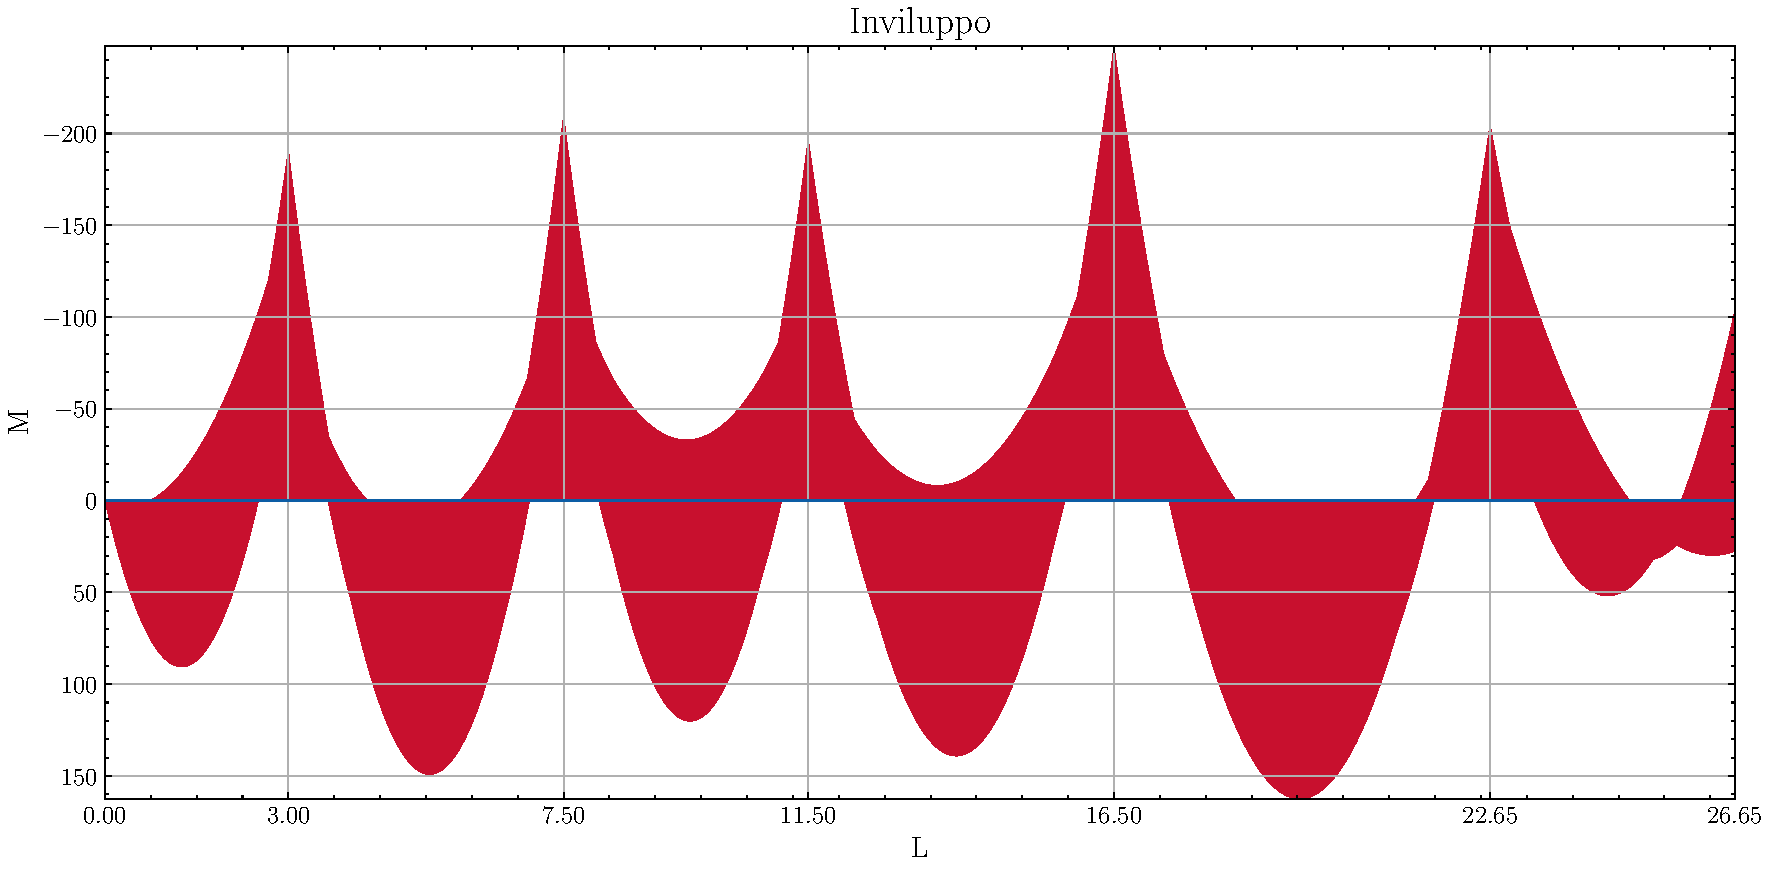
\includegraphics[height=0.6\textwidth]{IMG/diagrammi_trave/ULS_M.pdf}
\caption{Diagrammi del momento generati con combinazione di carico SLU}
\label{fig:trave_ULS_momento}
\end{figure}
\begin{table}[H]
\footnotesize
\centering
\caption{Valori del momento con combinazione di carico SLU nei punti più significativi della struttura}
\label{tab:trave_ULS_momento}
	\begin{tabular}{lS[table-format=-3.2]S[table-format=-3.2]S[table-format=-3.2]S[table-format=-3.2]S[table-format=-3.2]S[table-format=-3.2]S[table-format=-3.2]S[table-format=-3.2]S[table-format=-3.2]S[table-format=-3.2]S[table-format=-3.2]S[table-format=-3.2]S[table-format=-3.2]}
		\toprule
		{} & {A1} & {C1} & {A2} & {C2} & {A3} & {C3} & {A4} & {C4} & {A5} & {C5} & {A6} & {C6} & {A7} \\
		\midrule
		$s\,\si{[\metre]}$ & 0.00 & 1.26 & 3.00 & 5.31 & 7.50 & 9.57 & 11.50 & 13.92 & 16.50 & 19.54 & 22.65 & 24.57 & 26.65 \\
        $M^{-}\,\si{[\kilo\newton\metre]}$ & 0.00 & -15.14 & -190.97 & 0.00 & -209.46 & -33.15 & -196.60 & -10.06 & -247.45 & 0.00 & -204.82 & -18.04 & -103.04 \\
        $M^{+}\,\si{[\kilo\newton\metre]}$ & 0.00 & 90.60 & 0.00 & 149.18 & 0.00 & 120.20 & 0.00 & 139.16 & 0.00 & 162.53 & 0.00 & 51.88 & 27.68 \\
		\bottomrule
	\end{tabular}
\end{table}
\clearpage
\begin{figure}[H]
	\centering
	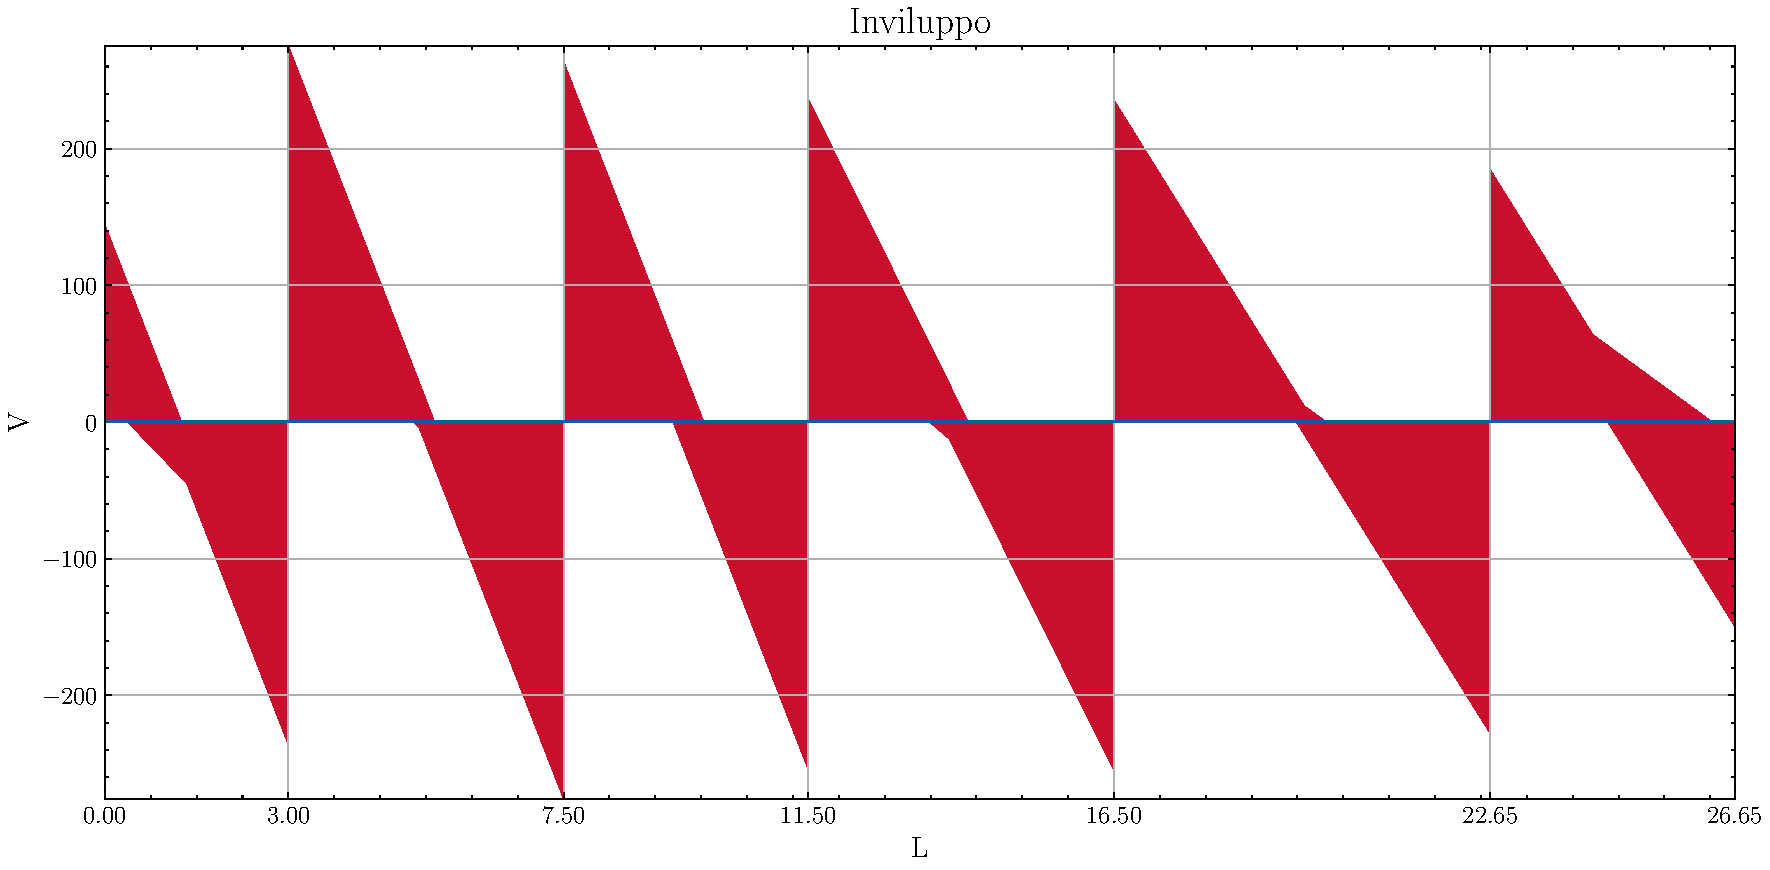
\includegraphics[height=0.6\textwidth]{IMG/diagrammi_trave/ULS_V.pdf}
	\caption{Diagrammi del taglio generati con combinazione di carico SLU}
	\label{fig:trave_ULS_taglio}
	\end{figure}
	\begin{table}[H]
	\footnotesize
	\centering
	\caption{Valori del taglio con combinazione di carico SLU nei punti più significativi della struttura}
	\label{tab:trave_ULS_taglio}
		\begin{tabular}{lS[table-format=-3.2]S[table-format=-3.2]S[table-format=-3.2]S[table-format=-3.2]S[table-format=-3.2]S[table-format=-3.2]S[table-format=-3.2]}
			\toprule
			{}                           & {A1}   & {A2}    & {A3}    & {A4}    & {A5}    & {A6}    & {A7} \\
			\midrule
			$s\,\si{[\metre]}$			 & 0.00   & 3.00    & 7.50    & 11.50   & 16.50   & 22.65   & 26.65 \\
			$V^{+}\,\si{[\kilo\newton]}$ & 144.22 & 275.03  & 263.72  & 236.15  & 235.45  & 184.80  & 0.00 \\
			$V^{-}\,\si{[\kilo\newton]}$ & 0.00   & -236.08 & -275.73 & -254.15 & -255.13 & -227.87 & -149.29 \\
			\bottomrule
		\end{tabular}
	\end{table}
%%%%%%%%%%%%%%%%%%%%%%%%%%%%%%%%%%%%%%%%%%%%%%%%%%%%%%%%%%%%%%%%%%%%%%%%%%%%%%%%
%%%%%%%%%%%%%%%%%%%%%%%%%%%%%%%%%%%%%%%%%%%%%%%%%%%%%%%%%%%%%%%%%%%%%%%%%%%%%%%%
%%%%%%%%%%%%%%%%%%%%%%%%%%%%%%%%%%%%%%%%%%%%%%%%%%%%%%%%%%%%%%%%%%%%%%%%%%%%%%%%
\clearpage
\subsection{SLS CHAR}
\begin{figure}[H]
\centering
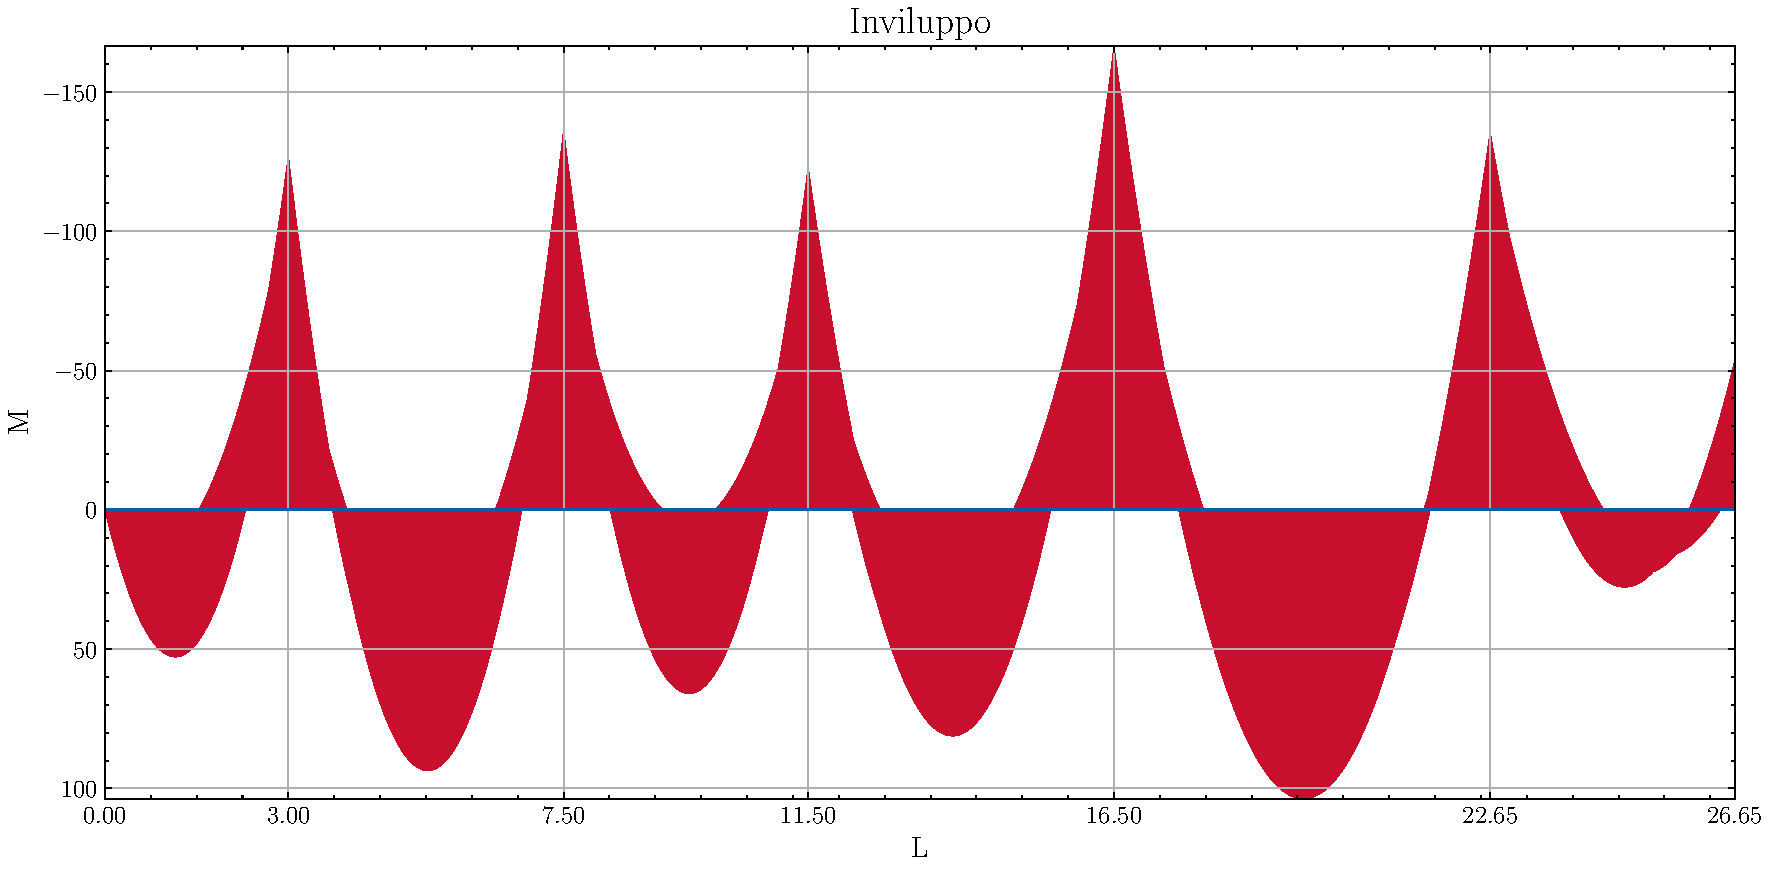
\includegraphics[height=0.6\textwidth]{IMG/diagrammi_trave/SLS_CHAR_M.pdf}
\caption{Diagrammi del momento generati con combinazione di carico SLS CHAR}
\label{fig:trave_SLS_CHAR_momento}
\end{figure}
\begin{table}[H]
\footnotesize
\centering
\caption{Valori del momento con combinazione di carico SLS CHAR nei punti più significativi della struttura}
\label{tab:trave_SLS_CHAR_momento}
	\begin{tabular}{lS[table-format=-3.2]S[table-format=-3.2]S[table-format=-3.2]S[table-format=-3.2]S[table-format=-3.2]S[table-format=-3.2]S[table-format=-3.2]S[table-format=-3.2]S[table-format=-3.2]S[table-format=-3.2]S[table-format=-3.2]S[table-format=-3.2]S[table-format=-3.2]}
		\toprule
		{} & {A1} & {C1} & {A2} & {C2} & {A3} & {C3} & {A4} & {C4} & {A5} & {C5} & {A6} & {C6} & {A7} \\
		\midrule
		$s\,\si{[\metre]}$ & 0.00 & 1.15 & 3.00 & 5.28 & 7.50 & 9.55 & 11.50 & 13.86 & 16.50 & 19.60 & 22.65 & 24.85 & 26.65 \\
        $M^{-}\,\si{[\kilo\newton\metre]}$ & 0.00 & 0.00 & -127.10 & 0.00 & -136.29 & 0.00 & -123.07 & 0.00 & -166.36 & 0.00 & -135.56 & 0.00 & -53.40 \\
        $M^{+}\,\si{[\kilo\newton\metre]}$ & 0.00 & 52.84 & 0.00 & 93.64 & 0.00 & 65.97 & 0.00 & 81.21 & 0.00 & 103.77 & 0.00 & 27.76 & 0.00 \\
		\bottomrule
	\end{tabular}
\end{table}
%%%%%%%%%%%%%%%%%%%%%%%%%%%%%%%%%%%%%%%%%%%%%%%%%%%%%%%%%%%%%%%%%%%%%%%%%%%%%%%%
%%%%%%%%%%%%%%%%%%%%%%%%%%%%%%%%%%%%%%%%%%%%%%%%%%%%%%%%%%%%%%%%%%%%%%%%%%%%%%%%
%%%%%%%%%%%%%%%%%%%%%%%%%%%%%%%%%%%%%%%%%%%%%%%%%%%%%%%%%%%%%%%%%%%%%%%%%%%%%%%%
\clearpage
\subsection{SLS FREQ}
\begin{figure}[H]
\centering
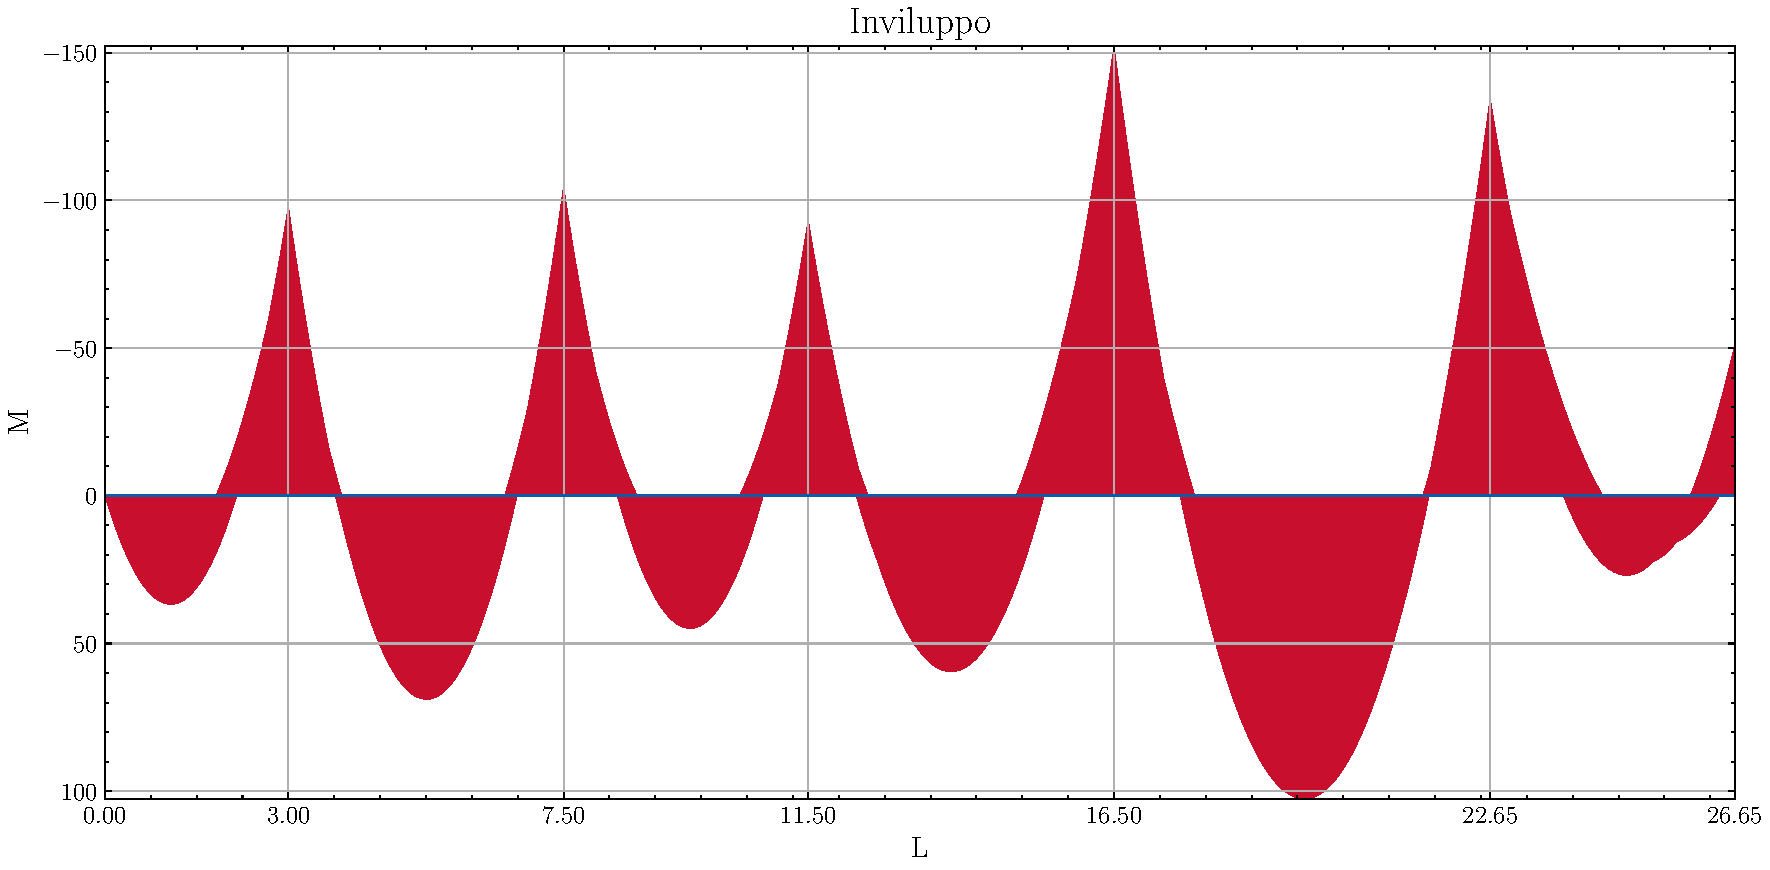
\includegraphics[height=0.6\textwidth]{IMG/diagrammi_trave/SLS_FREQ_M.pdf}
\caption{Diagrammi del momento generati con combinazione di carico SLS FREQ}
\label{fig:trave_SLS_FREQ_momento}
\end{figure}
\begin{table}[H]
\footnotesize
\centering
\caption{Valori del momento con combinazione di carico SLS FREQ nei punti più significativi della struttura}
\label{tab:trave_SLS_FREQ_momento}
	\begin{tabular}{lS[table-format=-3.2]S[table-format=-3.2]S[table-format=-3.2]S[table-format=-3.2]S[table-format=-3.2]S[table-format=-3.2]S[table-format=-3.2]S[table-format=-3.2]S[table-format=-3.2]S[table-format=-3.2]S[table-format=-3.2]S[table-format=-3.2]S[table-format=-3.2]}
		\toprule
		{} & {A1} & {C1} & {A2} & {C2} & {A3} & {C3} & {A4} & {C4} & {A5} & {C5} & {A6} & {C6} & {A7} \\
		\midrule
		$s\,\si{[\metre]}$ & 0.00 & 1.08 & 3.00 & 5.26 & 7.50 & 9.57 & 11.50 & 13.84 & 16.50 & 19.61 & 22.65 & 24.89 & 26.65 \\
        $M^{-}\,\si{[\kilo\newton\metre]}$ & 0.00 & 0.00 & -97.86 & 0.00 & -104.49 & 0.00 & -93.23 & 0.00 & -152.16 & 0.00 & -134.39 & 0.00 & -50.86 \\
        $M^{+}\,\si{[\kilo\newton\metre]}$ & 0.00 & 36.75 & 0.00 & 68.89 & 0.00 & 44.89 & 0.00 & 59.55 & 0.00 & 102.61 & 0.00 & 26.90 & 0.00 \\
		\bottomrule
	\end{tabular}
\end{table}
%%%%%%%%%%%%%%%%%%%%%%%%%%%%%%%%%%%%%%%%%%%%%%%%%%%%%%%%%%%%%%%%%%%%%%%%%%%%%%%%
%%%%%%%%%%%%%%%%%%%%%%%%%%%%%%%%%%%%%%%%%%%%%%%%%%%%%%%%%%%%%%%%%%%%%%%%%%%%%%%%
%%%%%%%%%%%%%%%%%%%%%%%%%%%%%%%%%%%%%%%%%%%%%%%%%%%%%%%%%%%%%%%%%%%%%%%%%%%%%%%%
\clearpage
\subsection{SLS QP}
\begin{figure}[H]
\centering
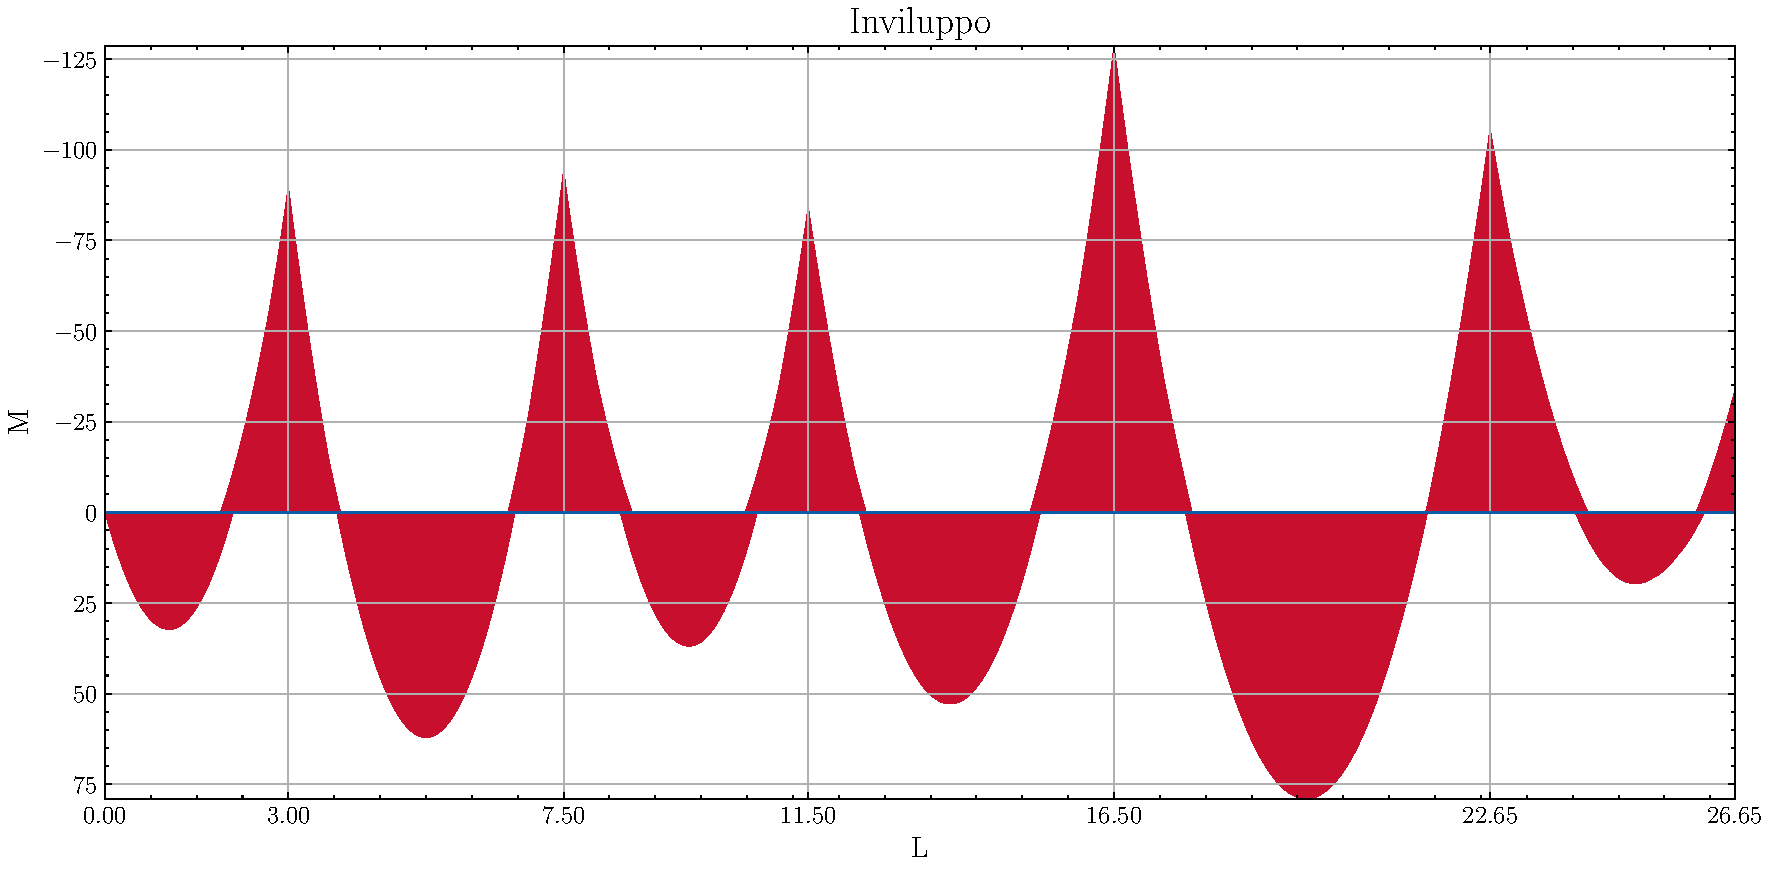
\includegraphics[height=0.6\textwidth]{IMG/diagrammi_trave/SLS_QP_M.pdf}
\caption{Diagrammi del momento generati con combinazione di carico SLS QP}
\label{fig:trave_SLS_QP_momento}
\end{figure}
\begin{table}[H]
\footnotesize
\centering
\caption{Valori del momento con combinazione di carico SLS QP nei punti più significativi della struttura}
\label{tab:trave_SLS_QP_momento}
	\begin{tabular}{lS[table-format=-3.2]S[table-format=-3.2]S[table-format=-3.2]S[table-format=-3.2]S[table-format=-3.2]S[table-format=-3.2]S[table-format=-3.2]S[table-format=-3.2]S[table-format=-3.2]S[table-format=-3.2]S[table-format=-3.2]S[table-format=-3.2]S[table-format=-3.2]}
		\toprule
		{} & {A1} & {C1} & {A2} & {C2} & {A3} & {C3} & {A4} & {C4} & {A5} & {C5} & {A6} & {C6} & {A7} \\
		\midrule
		$s\,\si{[\metre]}$ & 0.00 & 1.05 & 3.00 & 5.25 & 7.50 & 9.55 & 11.50 & 13.82 & 16.50 & 19.64 & 22.65 & 25.03 & 26.65 \\
        $M^{-}\,\si{[\kilo\newton\metre]}$ & 0.00 & 0.00 & -89.86 & 0.00 & -94.39 & 0.00 & -84.39 & 0.00 & -128.52 & 0.00 & -105.91 & 0.00 & -33.50 \\
        $M^{+}\,\si{[\kilo\newton\metre]}$ & 0.00 & 32.31 & 0.00 & 62.11 & 0.00 & 36.93 & 0.00 & 52.86 & 0.00 & 79.04 & 0.00 & 19.71 & 0.00 \\
		\bottomrule
	\end{tabular}
\end{table}

\end{landscape}

%{} & {A1} & {C1} & {A2} & {C2} & {A3} & {C3} & {A4} & {C4} & {A5} & {C5} & {A6} & {C6} & {A7} \\
%&\multicolumn{1}{c}{Nodo 1}&\multicolumn{1}{c}{Camp. 1}&\multicolumn{1}{c}{Nodo 2}&\multicolumn{1}{c}{Camp. 2}&\multicolumn{1}{c}{Nodo 3}&\multicolumn{1}{c}{Camp. 3}&\multicolumn{1}{c}{Nodo 4}&\multicolumn{1}{c}{Camp. 4}&\multicolumn{1}{c}{Nodo 5}&\multicolumn{1}{c}{Camp. 5}&\multicolumn{1}{c}{Nodo 6}&\multicolumn{1}{c}{Camp. 6}&\multicolumn{1}{c}{Nodo 7}\\
		

\section{Solaio}

\section{Pilastro}

\begin{figure}[htb]
	\centering
	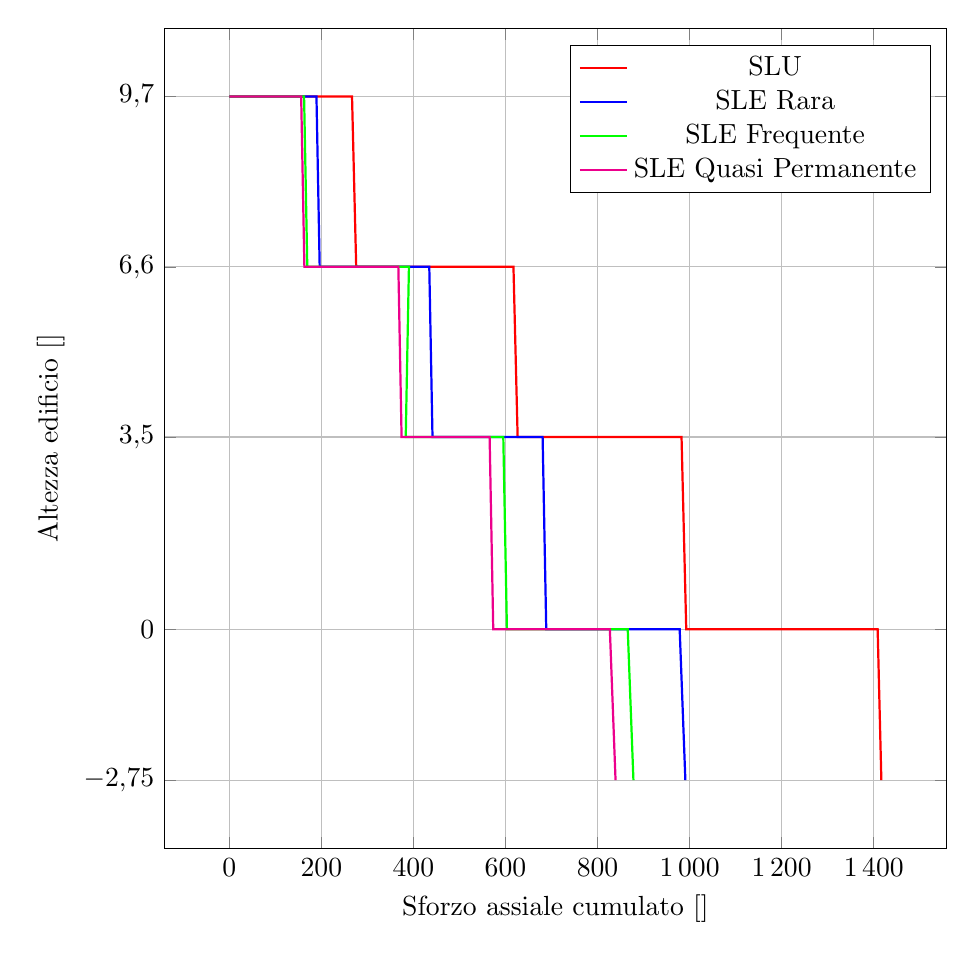
\begin{tikzpicture}
		\begin{axis}[
			/pgf/number format/.cd,
			use comma,      %virgola nei decimali
			1000 sep={\,},  %uno spazio nelle migliaia
			height=12cm,
			width=0.95\textwidth,
			grid=major,
			xlabel=Sforzo assiale cumulato \si{[\kilo\newton]},
			ylabel=Altezza edificio \si{[\meter]},
			ytick = {9.7,6.6,3.5,0,-2.75},
			%title=Titolo se serve
		]
		\addplot[thick,color=red] coordinates {
		   (0000.00, 9.7  )
		   (0266.64, 9.7  )
		   (0275.70, 6.6  )
		   (0617.34, 6.6  )
		   (0626.41, 3.5  )
		   (0982.45, 3.5  )
		   (0992.69, 0    )
		   (1408.49, 0    )
		   (1416.53, -2.75)
		};
		\addplot[thick,color=blue] coordinates {
		   (0000.00,  9.7  )
		   (0189.40, 9.7  )
		   (0196.37, 6.6  )
		   (0434.48, 6.6  )
		   (0441.45, 3.5  )
		   (0680.68, 3.5  )
		   (0688.56, 0    )
		   (0978.41, 0    )
		   (0990.79, -2.75)
		};
		\addplot[thick,color=green] coordinates {
		   (0000.00,  9.7  )
		   (0162.48, 9.7  )
		   (0169.45, 6.6  )
		   (0390.28, 6.6  )
		   (0383.31, 3.5  )
		   (0595.26, 3.5  )
		   (0603.13, 0    )
		   (0865.58, 0    )
		   (0877.96, -2.75)
		};
		\addplot[thick,color=magenta] coordinates {
		   (0000.00,  9.7  )
		   (0156.17, 9.7  )
		   (0163.15, 6.6  )
		   (0367.30, 6.6  )
		   (0374.28, 3.5  )
		   (0565.55, 3.5  )
		   (0573.42, 0    )
		   (0826.74, 0    )
		   (0839.11, -2.75)
		};
		\legend{SLU,SLE Rara,SLE Frequente,SLE Quasi Permanente}
		\end{axis}
	\end{tikzpicture}
	\caption{Andamento dello sforzo assiale agente sul pilastro P27 in funzione dell'altezza}
	\label{fig:AndamentoP27}
	\end{figure}